\documentclass[runningheads]{llncs}
\usepackage[T1]{fontenc}
\usepackage{graphicx}
\usepackage{amsmath,amssymb,amsfonts}
\usepackage{booktabs}
\usepackage{multirow}
\usepackage{array}
\usepackage{cite}
\usepackage{hyperref}
\hypersetup{hidelinks=true}

% --- global table styling: airy, professional spacing on every table ---
\renewcommand{\arraystretch}{1.02}
\setlength{\tabcolsep}{6pt}

% --- relax float placement so figures/tables are not deferred to the end
% (prevents blank space + content spilling onto an extra page) ---
\renewcommand{\topfraction}{0.92}
\renewcommand{\bottomfraction}{0.85}
\renewcommand{\textfraction}{0.06}
\renewcommand{\floatpagefraction}{0.75}
\setcounter{topnumber}{3}
\setcounter{bottomnumber}{2}
\setcounter{totalnumber}{5}

\begin{document}

\title{A Domain-Split Mixture-of-Experts Framework for
Four-Class Mammography Lesion Detection on CBIS-DDSM}

\titlerunning{DS-MoE for Mammography Lesion Detection}

\author{Dhanraj Singh}

\authorrunning{D. Singh}

\institute{Department of Computer Science and Engineering,\\
Indian Institute of Technology Indore, Indore, India\\
\email{dhanraj.singh@iit.ac.in}}

\maketitle

%-----------------------------------------------------------------------
\begin{abstract}
Automated mammography screening must detect two radiologically distinct
lesion families---masses and calcifications---that differ sharply in
scale and detection difficulty. Masses are soft-tissue opacities
spanning tens to hundreds of pixels, whereas microcalcification clusters
collapse to a few pixels once a full-field mammogram is downscaled to a
1280-pixel network input, so training one detector jointly on all four
CBIS-DDSM classes forces a shared loss over fundamentally different
regimes. We propose a Domain-Split Mixture-of-Experts (DS-MoE) framework
that assigns dedicated YOLO11l detectors to the mass and calcification
domains and merges their predictions at inference through a
parameter-free class-offset union requiring no routing---a static,
gate-free special case of mixture-of-experts; a Gated MoE variant adds
a lightweight image-level router. To keep every comparison honest, all
experiments use patient-level GroupShuffleSplit partitions that
eliminate label leakage, and three seeds characterise variance. On the
458-image CBIS-DDSM test set, DS-MoE improves mAP50 by 13.9\% over a
leakage-free universal baseline ($0.0649 \pm 0.0114$ vs
$0.0570 \pm 0.0014$), with 27.0\% and 15.0\% gains on the two mass
classes, while aggregate Free-Response ROC sensitivity at two false
positives per image is unchanged ($0.2027$ vs $0.2021$); per-class FROC
sensitivity, however, favours the universal baseline---a
precision-for-sensitivity tradeoff we analyse in
Section~\ref{sec:discussion}. The advantage transfers zero-shot across
scanners without fine-tuning: mass FROC S@2 rises 11.6\% on INbreast,
mAP50 rises 4.2\% on MIAS, and a proxy image-level sensitivity on CMMD
rises from a near-zero baseline ($0.002$) to $0.155$. Controlled ablations further show
that CLAHE preprocessing is harmful for YOLO-based calcification
detection ($-38.6\%$ mAP50). We identify the calcification expert as the
resolution-limited system bottleneck. All absolute scores are
intentionally conservative, reflecting leakage-free evaluation on an
intrinsically hard full-field detection task.
\end{abstract}

\keywords{breast cancer screening \and calcification detection \and
CBIS-DDSM \and FROC analysis \and mammography lesion detection \and
mixture of experts \and object detection \and YOLO}

%-----------------------------------------------------------------------
\section{Introduction}
\label{sec:introduction}

Breast cancer remains the most frequently diagnosed malignancy in women
globally, with approximately 2.3 million new cases reported in 2020
\cite{sung2021global}. Mammographic screening has been shown to reduce
breast cancer mortality by detecting lesions at earlier, more treatable
stages \cite{tabar2003swedish}, and it remains the primary modality in
national screening programmes worldwide. Despite this, a meaningful
fraction of breast cancers are missed at initial reading. Retrospective
analyses consistently show that missed cancers fall into two distinct
visual categories: mass-like opacities that were present but overlooked,
and subtle microcalcification clusters that were not flagged
\cite{doi2007computer}. Computer-aided detection (CAD) systems are
intended to reduce these miss rates, yet translating benchmark
performance into clinical utility has proven harder than anticipated.

One structural reason is that mass and calcification lesions do not
share the same detection challenge. A mass occupies a recognisable blob
of tissue at multiple scales; its edges interact with surrounding
parenchyma in ways that can be captured by standard feature pyramid
representations. A microcalcification cluster, by contrast, may span
only 5--15 pixels in the original $3000 \times 4000$ pixel mammogram.
After network downscaling to a 1280-pixel input, those pixels collapse
to as few as one or two, below the reliable receptive field of any
standard convolutional anchor. This resolution mismatch is not merely a
data insufficiency problem; it is a structural mismatch between what the
network can represent and what the target looks like after preprocessing.

Most published CAD pipelines address multi-class mammography detection
by training a single model on all lesion categories simultaneously
\cite{ribli2018detecting}. The rationale is straightforward: a shared
backbone can reuse low-level features across lesion types, and joint
training is simpler to engineer. The cost is that the optimiser must
balance loss contributions from classes with very different difficulty
profiles. When calcification detection collapses at standard resolution,
the gradient signal from calc images provides little useful information
to the backbone, and the network effectively specialises on mass
detection by default---while still being penalised for calc misses.
This implicit bias is invisible in aggregate metrics but becomes apparent
when per-class results are examined.

Mixture-of-Experts (MoE) architectures \cite{jacobs1991adaptive} offer
a principled alternative: route inputs to specialist subnetworks, each
optimised for a well-defined subset of the problem. In sparse variants
\cite{shazeer2017outrageously} a hard top-$k$ selection activates only
the most relevant experts, allowing model capacity to scale without
proportional per-input compute overhead. These ideas have been applied
widely in natural language processing but have received limited
evaluation in medical object detection, where class heterogeneity is
severe and labelled data are scarce.

We investigate whether a simple domain-split MoE---one expert per
lesion family, no routing decision, predictions merged by class-offset
union---can improve four-class mammography detection on the CBIS-DDSM
benchmark \cite{lee2017curated}. To characterise the value of routing,
we also evaluate a Gated MoE variant that uses a lightweight image
classifier to modulate expert confidence scores before merging. All
models share an identical patient-level data split so that the
comparison is unconfounded by leakage. We evaluate on three seeds to
characterise variance, and assess zero-shot generalisation on INbreast
\cite{moreira2012inbreast}, MIAS, and CMMD.

The main contributions of this paper are as follows:
\begin{enumerate}
\setlength{\itemsep}{0pt}
\setlength{\parskip}{0pt}
\item We introduce the Domain-Split MoE (DS-MoE) framework for
  four-class mammography detection, where specialist YOLO11l detectors
  for mass and calcification domains are trained independently and merged
  at inference through a parameter-free class-offset union (a static,
  gate-free special case of MoE)---achieving 13.9\% higher mAP50 than a
  leakage-free universal baseline with mass class gains of 27.0\% and
  15.0\%, while aggregate FROC S@2 remains equivalent (per-class
  sensitivity favours the baseline; Section~\ref{sec:discussion}).
\item We present, to our knowledge, the first patient-level
  leakage-free evaluation of a mixture-of-experts mammography detector
  across three external datasets (INbreast, MIAS, CMMD), showing
  zero-shot cross-scanner generalisation ($+11.6\%$ mass FROC S@2 on
  INbreast, and a proxy image-level sensitivity on CMMD recovered from a
  near-zero baseline $0.002$ to $0.155$).
\item We diagnose per-class FROC regression in DS-MoE as a consequence
  of cross-domain false-positive inflation from the calc expert, and
  quantify the tradeoff between mAP50 gains and per-class sensitivity.
\item We demonstrate through controlled ablation that CLAHE preprocessing
  is harmful for YOLO-based calcification detection on CBIS-DDSM
  ($-38.6\%$ mAP50), a negative result directly actionable for
  practitioners building mammography CAD pipelines.
\end{enumerate}

%-----------------------------------------------------------------------
\section{Related Work}
\label{sec:related}

\subsection{Mammography CAD and Lesion Detection}

Computer-aided detection in mammography predates deep learning by two
decades \cite{doi2007computer}. Classical pipelines combined
Laplacian-of-Gaussian blob detectors for calcification clusters with
morphological and rule-based classifiers for mass shape and BI-RADS
assessment, but degraded substantially across scanner vendors and
acquisition protocols, limiting clinical adoption.

The release of CBIS-DDSM \cite{lee2017curated} and INbreast
\cite{moreira2012inbreast} made large-scale convolutional approaches
tractable. Ribli \textit{et al.} \cite{ribli2018detecting} applied a
Faster R-CNN variant to DDSM images and demonstrated that end-to-end
detection networks could approach radiologist sensitivity on held-out
cases. Since then, feature pyramid networks, multi-scale attention, and
self-supervised pre-training have progressively improved benchmark
numbers. A persistent challenge across all these methods is severe class
imbalance between benign and malignant subtypes, which biases models
toward majority classes even when minority-class recall is clinically
more important. Generalisation across acquisition modalities---screen-film
to full-field digital---remains non-trivial, reflecting distributional
shift in image contrast, noise characteristics, and glandular density.

A critical but often overlooked issue in the literature is data leakage.
Many papers split CBIS-DDSM at the image level, inadvertently placing
views of the same patient in both train and test partitions. Lee
\textit{et al.} \cite{lee2017curated} explicitly warn that image-level
splits can inflate detection metrics by 30--50\% or more, making honest
cross-paper comparison impossible. Our work enforces strict patient-level
partitioning via \texttt{GroupShuffleSplit} throughout all experiments;
direct numerical comparison with prior work is therefore not meaningful
and is not attempted.

\subsection{YOLO-Based Detection in Medical Imaging}

The YOLO family of single-stage detectors \cite{redmon2016you} has
gained traction in medical imaging applications due to its inference
speed and competitive accuracy. YOLOv8 and YOLO11 \cite{jocher2024ultralytics}
use path aggregation network necks with multi-scale prediction heads at
strides 8, 16, and 32. The optional P2 head adds a stride-4 output
specifically for very small objects, and has shown utility in satellite
imagery and digital pathology where the object-to-image area ratio is
extremely low. Applied to full-field mammography, YOLO-based detectors
face the challenge that calcification clusters occupy a negligible
fraction of image area after downscaling, while masses are more
amenable to standard anchor-based detection.

Sliced Inference with Hyper Inference (SAHI) \cite{akyon2022sahi}
addresses small-object detection at inference time by dividing the
input into overlapping tiles, running the detector on each tile
independently, and merging predictions with non-maximum suppression.
This recovers detections lost after global downscaling, at the cost of
inference time proportional to tile count. For mammography calcification
clusters, SAHI is a natural candidate to address the resolution
bottleneck identified in this work; we evaluate tiling as a direction
in Section~\ref{sec:discussion} and leave full SAHI integration to
future work.

\subsection{Mixture-of-Experts for Vision}

The MoE framework of Jacobs \textit{et al.} \cite{jacobs1991adaptive}
trained specialist networks with a gating network that assigned input
samples to the most relevant expert via soft weighting. Shazeer
\textit{et al.} \cite{shazeer2017outrageously} introduced sparse
top-$k$ gating that scales MoE model capacity without proportional
compute cost, enabling the very large MoE transformers now common in
NLP. In vision, MoE has been applied mainly to classification and scene
understanding tasks. Applying hard routing to object detection is
complicated because a single image can contain lesions from multiple
classes, so assigning the entire image to one expert risks suppressing
detections from the other. Our Domain-Split approach avoids this by
running all experts on every image and merging by class partition,
making it robust to images that contain both mass and calcification
lesions simultaneously. We use ``mixture-of-experts'' in the sense of
specialised subnetworks combined at inference: DS-MoE is deliberately a
hard, static domain partition rather than a learned gate, and the Gated
MoE variant (Section~\ref{sec:method}) isolates the effect of adding
learned routing on top of this partition.

%-----------------------------------------------------------------------
\section{Dataset}
\label{sec:dataset}

\subsection{CBIS-DDSM}

The Curated Breast Imaging Subset of DDSM (CBIS-DDSM)
\cite{lee2017curated} contains digitised screen-film mammograms with
standardised ROI bounding box annotations for masses and calcification
clusters. We work with a four-class lesion detection formulation:
\textit{benign\_mass} (BM), \textit{malignant\_mass} (MM),
\textit{benign\_calc} (BC), and \textit{malignant\_calc} (MC). After
cleaning duplicate records and resolving filename collisions, the
dataset contains 3,242 usable records, of which 3,103 enter the
canonical\_4class partition (Table~\ref{tab:dataset}) after removing
images without valid four-class bounding-box annotations in YOLO
format. The fixed test partition used in all experiments contains 458
images with 518 ground-truth bounding boxes: BM = 147, MM = 106,
BC = 164, MC = 101. Calcification
annotations delineate the bounding box of the entire cluster, not
individual specks---an important distinction when comparing to external
datasets in Section~\ref{sec:external}.

\subsection{Patient-Level Split}

\begin{table}[tb]
\caption{Dataset partitions used in all experiments. Expert subsets
(canonical\_mass, canonical\_calc) use their own val sets during
training; all system-level results report on the shared 458-image
canonical\_4class test set.}
\label{tab:dataset}
\centering
\begin{tabular}{lcccc}
\toprule
\textbf{Subset} & \textbf{Classes} & \textbf{Train} & \textbf{Val} & \textbf{Test}\\
\midrule
canonical\_mass   & BM, MM         & 604  &  26 &  26\\
canonical\_calc   & BC, MC         & 483  &  17 &  18\\
canonical\_4class & BM, MM, BC, MC & 2190 & 455 & 458\\
canonical\_router & mass / calc    & 760  & 162 & 165\\
\bottomrule
\end{tabular}
\end{table}

All four subsets in Table~\ref{tab:dataset} derive from a single
patient-level \texttt{GroupShuffleSplit} \cite{pedregosa2011scikit}
with 80/10/10 train/val/test ratio applied at the patient identifier
level. Every patient identifier appears in exactly one partition,
preventing label leakage. The split uses seed 42 as the master
partition; all three experimental seeds (42, 1, 123) produce
independently trained models but evaluate on the same 458-image test
patients, ensuring a fair comparison. With $n=3$ pairs the minimum
achievable Wilcoxon signed-rank $p$-value is 0.25; we therefore do not
claim statistical significance and report mean $\pm$ population standard
deviation throughout.

%-----------------------------------------------------------------------
\section{Methodology}
\label{sec:method}

\subsection{Problem Formulation}

We formulate mammography lesion detection as a four-class object
detection problem over full-field mammograms. Given an input image
$\mathbf{x} \in \mathbb{R}^{H \times W}$ representing a single
mammographic view, the goal is to produce a set of predictions
$\mathcal{P} = \{(b_i, c_i, s_i)\}$ where $b_i$ is a bounding box,
$c_i \in \{0,1,2,3\}$ is the class index (BM, MM, BC, MC), and $s_i$
is the detection confidence score. The challenge is that the four
classes span two fundamentally different detection regimes: mass lesions
(classes 0--1) are blob-like objects at centimetre scale, while
calcification clusters (classes 2--3) are point-like objects at
millimetre scale that become sub-pixel after standard network
downscaling. A single shared model must balance these regimes; our
framework addresses this by domain splitting.

\subsection{Data Preparation}

Each canonical subset is constructed by filtering CBIS-DDSM records
for the relevant lesion types and converting bounding box annotations
to YOLO format (normalised $x_c, y_c, w, h$ per image). For
canonical\_mass and canonical\_calc, class indices are reassigned to a
local two-class scheme: BM/MM $\rightarrow$ 0/1 for mass, and
BC/MC $\rightarrow$ 0/1 locally for calc. At inference, a fixed offset
of $+2$ maps calc-expert predictions back to the global four-class
index space. Images are converted to 8-bit grayscale and saved as JPEG.
No CLAHE preprocessing is applied; Section~\ref{sec:ablation} shows
that CLAHE is harmful for YOLO-based calcification detection. Expert
model selection during training uses the expert's own val partition
(26 images for mass, 17 for calc); all final system-level comparisons
use the shared 458-image canonical\_4class test set.

\subsection{Expert Detector Training}

Both specialist detectors use YOLO11l \cite{jocher2024ultralytics}, a
large-scale single-stage detector with a path aggregation network neck
and multi-scale prediction heads at strides 8, 16, and 32. The input
resolution is set to 1280 pixels for all models to maximise mass
lesion visibility while remaining within GPU memory constraints on
NVIDIA T4 hardware (batch size 16, AMP enabled).

Training uses the AdamW optimiser with initial learning rate
$\eta_0 = 5 \times 10^{-4}$, cosine annealing to $\eta_f = \eta_0
\times 10^{-2}$, weight decay $\lambda = 5 \times 10^{-4}$, and
10-epoch linear warmup. Early stopping monitors validation mAP50 with
patience 30 over a maximum of 150 epochs.

Augmentation is domain-adapted: horizontal and vertical flip
(probability 0.5 each), colour jitter, and copy-paste ($p = 0.3$).
Mosaic augmentation is disabled for the calc expert because it
concatenates four images, disrupting the spatial density of
calcification clusters and artificially increasing background
complexity. Mosaic does not affect mass detection and is left at
default for other models.

The \textit{universal baseline} is a YOLO11l trained on the full
canonical\_4class partition (2190 images, four classes) with the
identical training configuration. This represents the conventional
single-model approach that jointly optimises all four classes.

Expert validation performance (mean over three seeds) is summarised in
Table~\ref{tab:expert_val}. These scores are computed on small
expert-specific partitions (26 and 17 images) and are therefore
high-variance and optimistic relative to the shared 458-image test set;
they indicate relative expert quality, not expected test performance,
which the substantially lower per-class test scores in
Table~\ref{tab:perclass} confirm.

\begin{table}[tb]
\caption{Expert detector validation mAP50 (mean, three seeds). The mass
and calc experts are evaluated on their own val partitions (26 and 17
images); the Universal row is evaluated on the 455-image four-class val
partition. These small-partition scores are high-variance and optimistic
relative to the 458-image test set (Tables~\ref{tab:main}--\ref{tab:perclass}).}
\label{tab:expert_val}
\centering
\begin{tabular}{lclc}
\toprule
\textbf{Expert} & \textbf{mAP50} & \textbf{Per-class AP50} & \textbf{Epochs}\\
\midrule
Mass Expert  & 0.499 & BM 0.264 \quad MM 0.734 & $\sim$107\\
Calc Expert  & 0.167 & BC 0.189 \quad MC 0.145 & $\sim$127\\
Universal    & 0.062 & BM 0.066 \quad MM 0.124 \quad BC 0.014 \quad MC 0.024 & $\sim$90\\
\bottomrule
\end{tabular}
\end{table}

\subsection{Domain-Split MoE Inference}

\begin{figure}[t]
\centerline{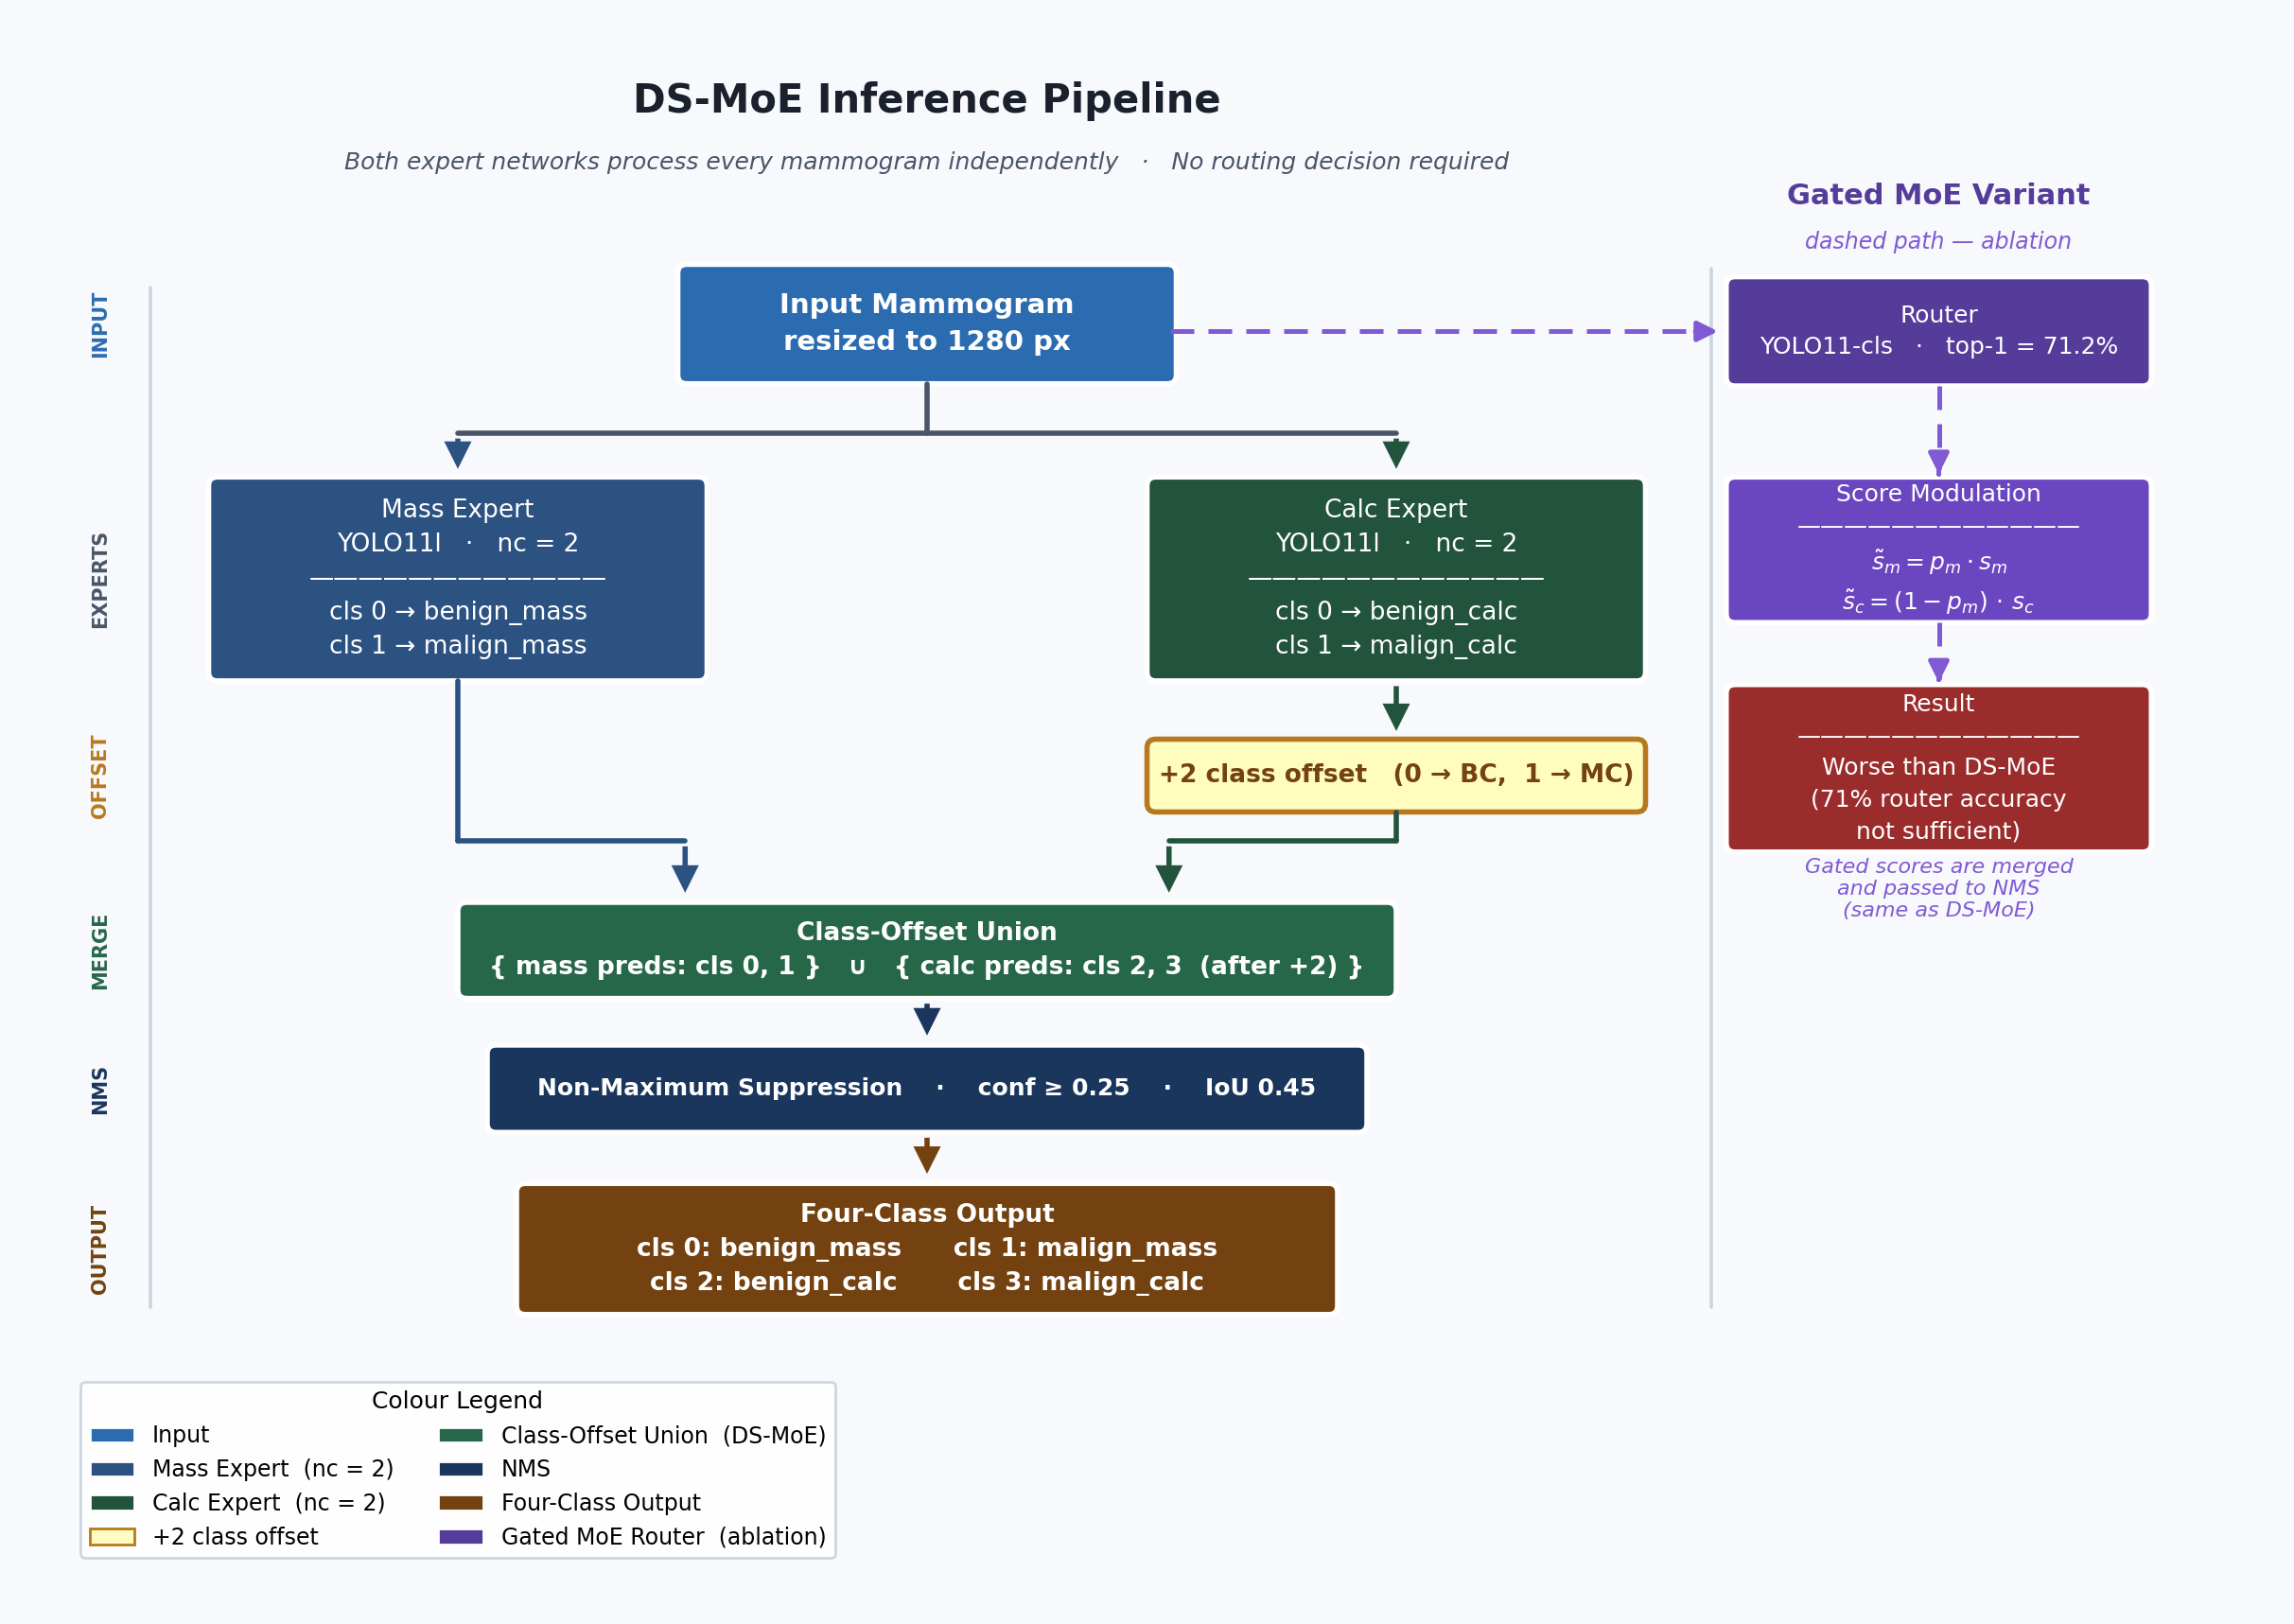
\includegraphics[width=\columnwidth]{pipeline_diagram.png}}
\caption{DS-MoE inference pipeline. Both expert detectors run on every
input mammogram independently. Calc expert predictions are remapped to
global classes 2--3 via a fixed $+2$ class offset. Predictions are
concatenated and filtered with NMS. The Gated MoE variant (dashed path)
modulates confidence scores using router probabilities
$\tilde{s}_{m,i} = p_m \cdot s_{m,i}$ before merging.}
\label{fig:pipeline}
\end{figure}

At inference, the mass expert and calc expert both process every test
image independently, as illustrated in Fig.~\ref{fig:pipeline}. Their
prediction sets are concatenated after applying the class offset: mass
expert predictions retain local class indices 0 (BM) and 1 (MM); calc
expert predictions are remapped to global classes 2 (BC) and 3 (MC)
by adding the fixed offset $+2$. Because the two class ranges are
disjoint, no ambiguity arises in the merged output. Standard
confidence-threshold filtering ($\tau = 0.25$) and non-maximum
suppression (IoU threshold 0.45) are then applied to the merged
prediction set.

DS-MoE requires no routing decision and therefore avoids routing
errors entirely. Its computational cost is that both expert networks
run at every inference step, doubling FLOPs relative to the universal
baseline.

\subsection{Gated MoE with Router}

The Gated MoE introduces a lightweight router to modulate expert
confidence scores before merging. The router is a YOLO11 classification
model trained on canonical\_router (760 training images, binary labels:
mass-dominant vs.\ calcification-dominant) for 50 epochs. It achieves
mean top-1 accuracy of 0.712 across three seeds (individual seeds:
0.710, 0.710, 0.716).

Let $s_{m,i}$ denote the confidence of the $i$-th prediction from the
mass expert and $p_m \in [0,1]$ the router probability for the mass
class. Modulated scores are computed as:
\begin{equation}
  \tilde{s}_{m,i} = p_m \cdot s_{m,i}, \quad
  \tilde{s}_{c,j} = (1 - p_m) \cdot s_{c,j},
  \label{eq:gating}
\end{equation}
where $s_{c,j}$ is the $j$-th calc expert prediction score. The
merged set $\{\tilde{s}_{m,i}\} \cup \{\tilde{s}_{c,j}\}$ is then
processed identically to DS-MoE with the same confidence threshold
and NMS parameters. In principle, gating suppresses predictions from
the non-dominant expert for each image; in practice, as
Section~\ref{sec:results} shows, the 71.2\% router accuracy is
insufficient to provide reliable modulation across the full test
distribution.

\subsection{Evaluation Protocol}

Two metrics are reported throughout. Mean average precision at IoU
threshold 0.50 (mAP50) is computed using the standard 101-point
interpolated precision-recall curve aggregated over all four classes;
we also report mAP50-95, the COCO-style mean of mAP over IoU thresholds
0.50 to 0.95 in steps of 0.05. FROC sensitivity at two false positives
per image (S@2) is computed with an IoU matching threshold of 0.30,
which reflects the lower localisation precision acceptable in clinical
screening CAD and follows the lenient-matching convention common in
mammography detection challenges.
Per-class variants of both metrics are computed by treating each class
separately. All evaluations run on the fixed 458-image CBIS-DDSM
test set with the 518 ground-truth bounding boxes described in
Section~\ref{sec:dataset}.

%-----------------------------------------------------------------------
\section{Experiments}
\label{sec:experiments}

\subsection{Implementation Details}

All models are trained using the Ultralytics YOLO11 framework
\cite{jocher2024ultralytics} on NVIDIA T4 GPUs (14.9 GB VRAM) via the
Kaggle platform. Mixed precision (AMP/FP16) is enabled throughout.
Each seed produces independently initialised model weights; no weight
sharing occurs across seeds or across expert/universal models within
a seed.

\subsection{Main Results}
\label{sec:results}

\begin{table}[tb]
\caption{Main comparison on the 458-image CBIS-DDSM test set
(mean $\pm$ std, three seeds 42/1/123). All models use identical
patient-level splits; direct comparison with prior work using
image-level splits is not meaningful (see Sec.~\ref{sec:related}).}
\label{tab:main}
\centering
\begin{tabular}{lccc}
\toprule
\textbf{Model} & \textbf{mAP50} & \textbf{mAP50-95} & \textbf{FROC S@2}\\
\midrule
Universal    & $0.0570 \pm 0.0014$ & $0.0243 \pm 0.0003$ & $0.2021 \pm 0.0071$\\
DS-MoE       & $\mathbf{0.0649 \pm 0.0114}$ & $\mathbf{0.0300 \pm 0.0049}$ & $0.2027 \pm 0.0114$\\
Gated MoE    & $0.0589 \pm 0.0075$ & $0.0263 \pm 0.0034$ & $0.1950 \pm 0.0150$\\
\midrule
\multicolumn{4}{l}{\small $\Delta$ DS-MoE vs Universal: mAP50 +13.9\%; FROC S@2 +0.3\%}\\
\bottomrule
\end{tabular}
\end{table}

Table~\ref{tab:main} reports the main comparison. DS-MoE achieves mean
mAP50 of $0.0649$, a 13.9\% improvement over Universal ($0.0570$),
driven entirely by mass class gains. Absolute mAP50 values are low
across all models, and we do not attribute this to any single cause.
Strict patient-level evaluation removes the label leakage that can
inflate image-level-split benchmarks by 30--50\% \cite{lee2017curated},
but leakage removal alone does not account for the magnitude: full-field
four-class detection is intrinsically hard, patient-level splitting
reduces the effective training set, and the difficult calcification
classes depress the four-class mean (Table~\ref{tab:perclass}). These numbers should therefore be read as controlled relative
comparisons under identical conditions, not as absolute capability and
not against leaked-split literature. Aggregate FROC S@2 is $0.2027$
for DS-MoE versus $0.2021$ for Universal---a difference of $0.0006$
far below any meaningful clinical threshold, confirming no aggregate
regression in detection completeness (Fig.~\ref{fig:froc}). Gated MoE
scores below DS-MoE on both metrics: with 71.2\% router accuracy,
incorrectly classified images have their correct expert down-weighted,
causing true positive boxes to fall below the confidence threshold
after gating.

\begin{figure}[t]
\centering
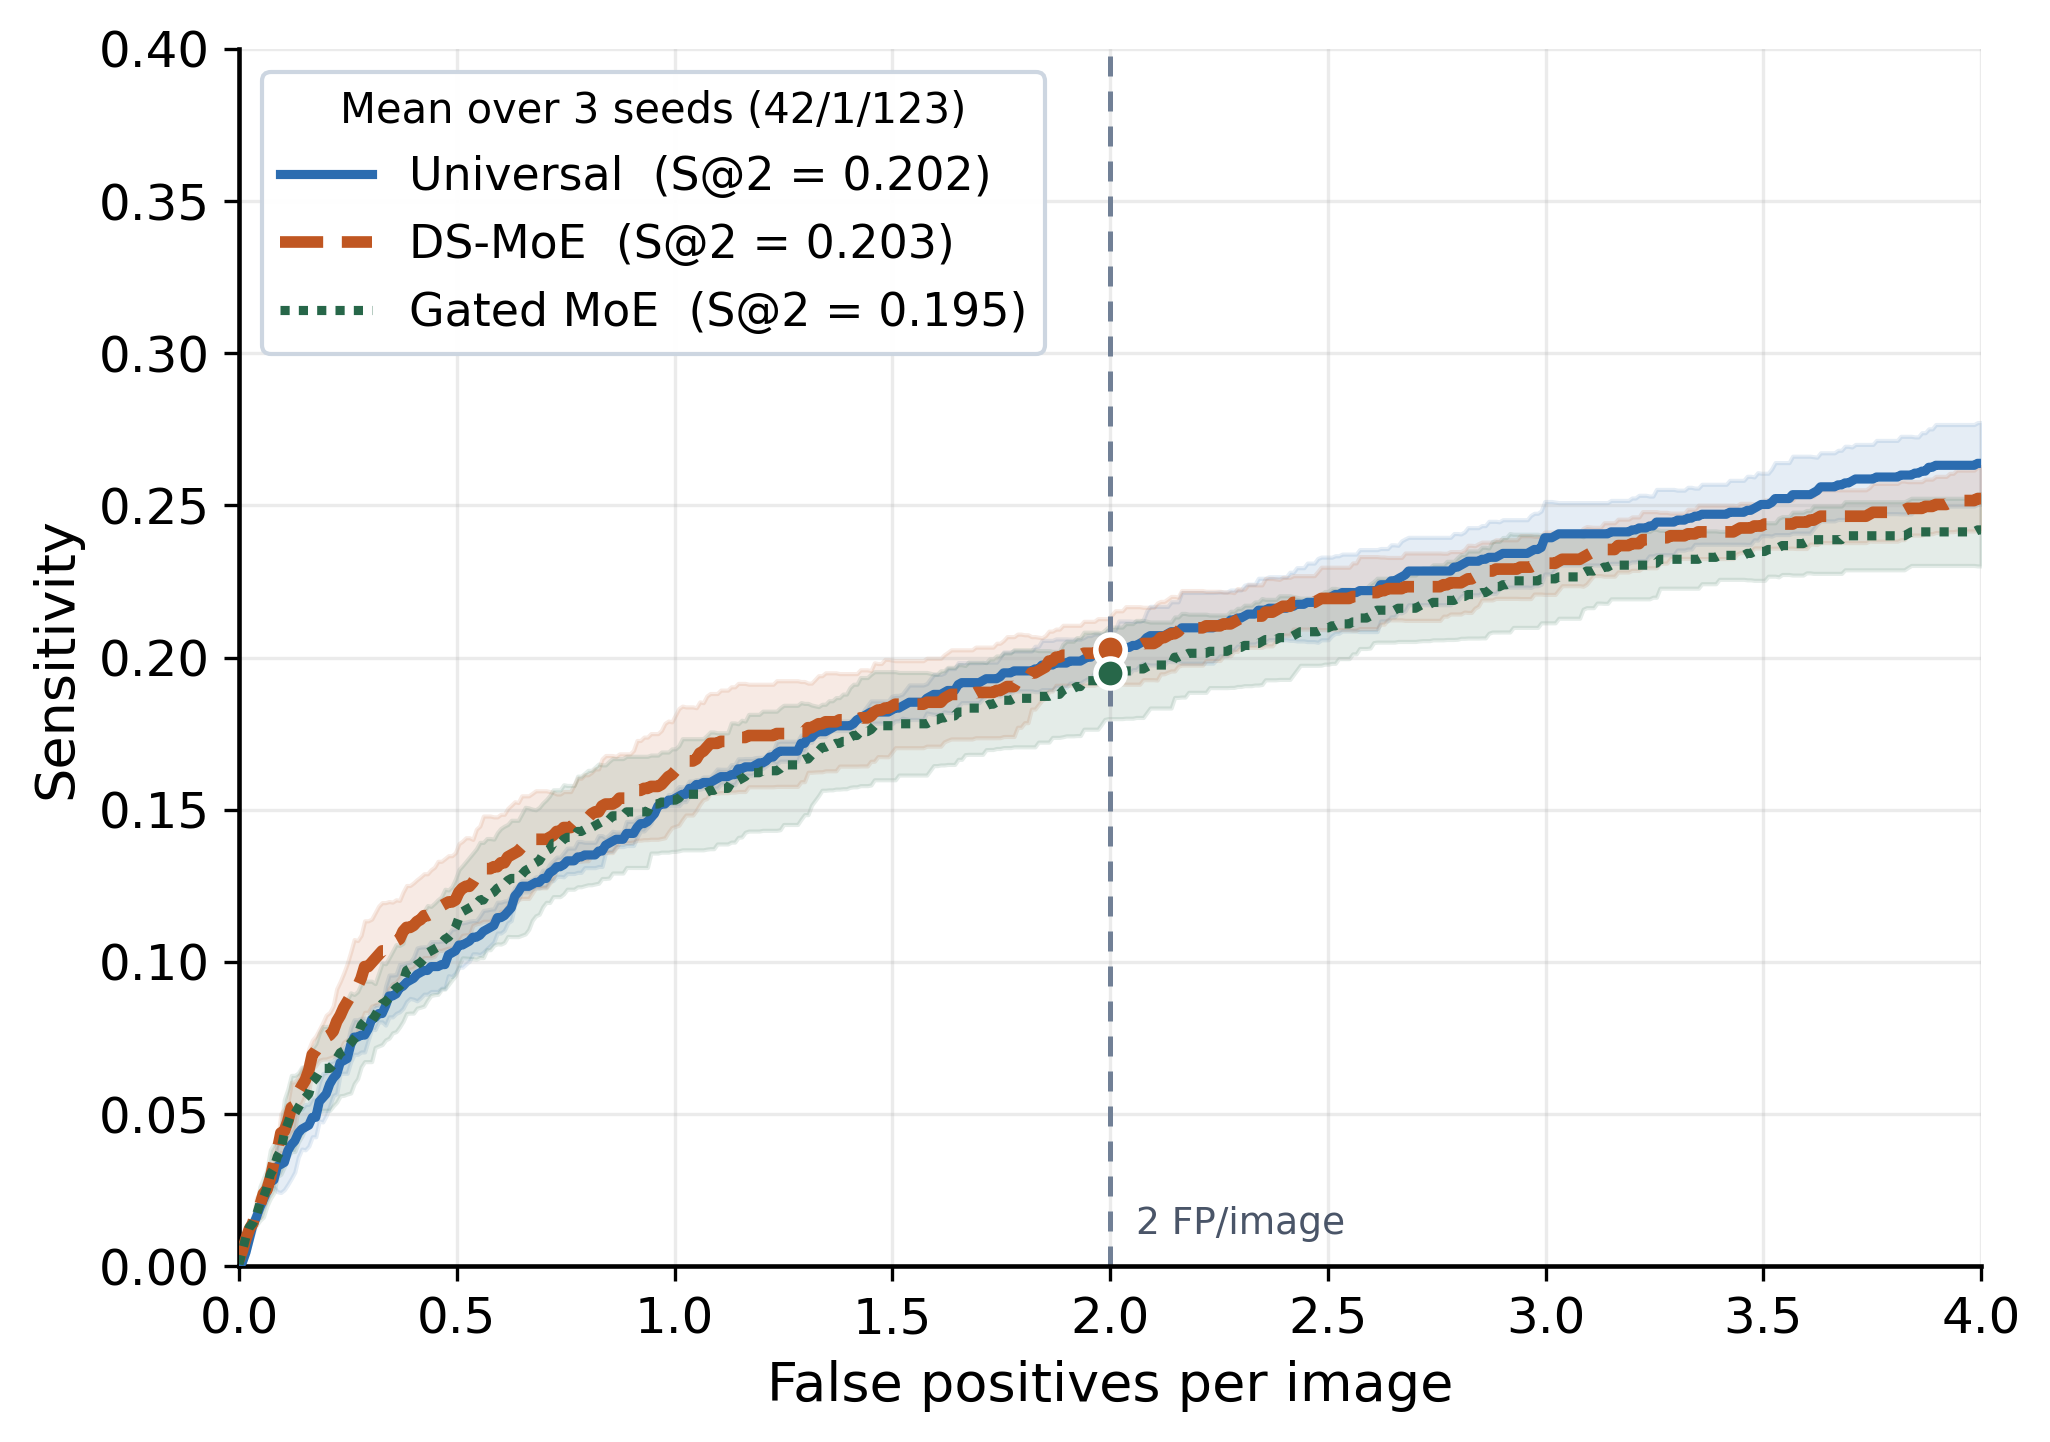
\includegraphics[width=0.78\columnwidth]{froc_curves.png}
\caption{FROC curves on the 458-image CBIS-DDSM test set (class-aware
matching, IoU matching threshold $=0.30$; mean over three seeds, shaded
band $=\pm1$ standard deviation). At the clinically relevant operating
point of two false positives per image (dashed line), the three models
are statistically indistinguishable (S@2 $=0.202$, $0.203$, and $0.195$
for Universal, DS-MoE, and Gated MoE respectively), confirming that
domain splitting introduces no aggregate sensitivity regression.
Absolute sensitivity is conservative: patient-level leakage-free
evaluation, together with the intrinsic difficulty of full-field
detection, yields lower numbers than the image-level splits common in
prior work.}
\label{fig:froc}
\end{figure}

\subsection{Per-Class Analysis}

\begin{table}[tb]
\caption{Per-class mAP50 (mean over three seeds). Bold = best per
column. DS-MoE gains are concentrated in mass classes.}
\label{tab:perclass}
\centering
\begin{tabular}{lcccc}
\toprule
\textbf{Model} & \textbf{Ben. Mass} & \textbf{Mal. Mass}
               & \textbf{Ben. Calc} & \textbf{Mal. Calc}\\
\midrule
Universal  & 0.0664 & 0.1236 & \textbf{0.0144} & 0.0237\\
DS-MoE     & \textbf{0.0843} & \textbf{0.1421} & 0.0099 & 0.0234\\
Gated MoE  & 0.0802 & 0.1133 & 0.0082 & \textbf{0.0338}\\
\midrule
$\Delta$ DS-MoE & $+$27.0\% & $+$15.0\% & $-$31.3\% & $-$1.3\%\\
\bottomrule
\end{tabular}
\end{table}

\begin{table}[tb]
\caption{Per-class FROC S@2 (mean over three seeds, IoU matching
threshold = 0.30). Universal achieves higher per-class sensitivity;
the aggregate tie in Table~\ref{tab:main} is explained by FP
inflation analysis in Section~\ref{sec:discussion}.}
\label{tab:perclass_froc}
\centering
\begin{tabular}{lcccc}
\toprule
\textbf{Model} & \textbf{Ben. Mass} & \textbf{Mal. Mass}
               & \textbf{Ben. Calc} & \textbf{Mal. Calc}\\
\midrule
Universal  & \textbf{0.4331} & \textbf{0.5377} & \textbf{0.2215} & \textbf{0.2937}\\
DS-MoE     & 0.3696 & 0.4340 & 0.1972 & 0.2574\\
Gated MoE  & 0.3673 & 0.4308 & 0.1728 & 0.2706\\
\bottomrule
\end{tabular}
\end{table}

\begin{figure}[t]
\centering
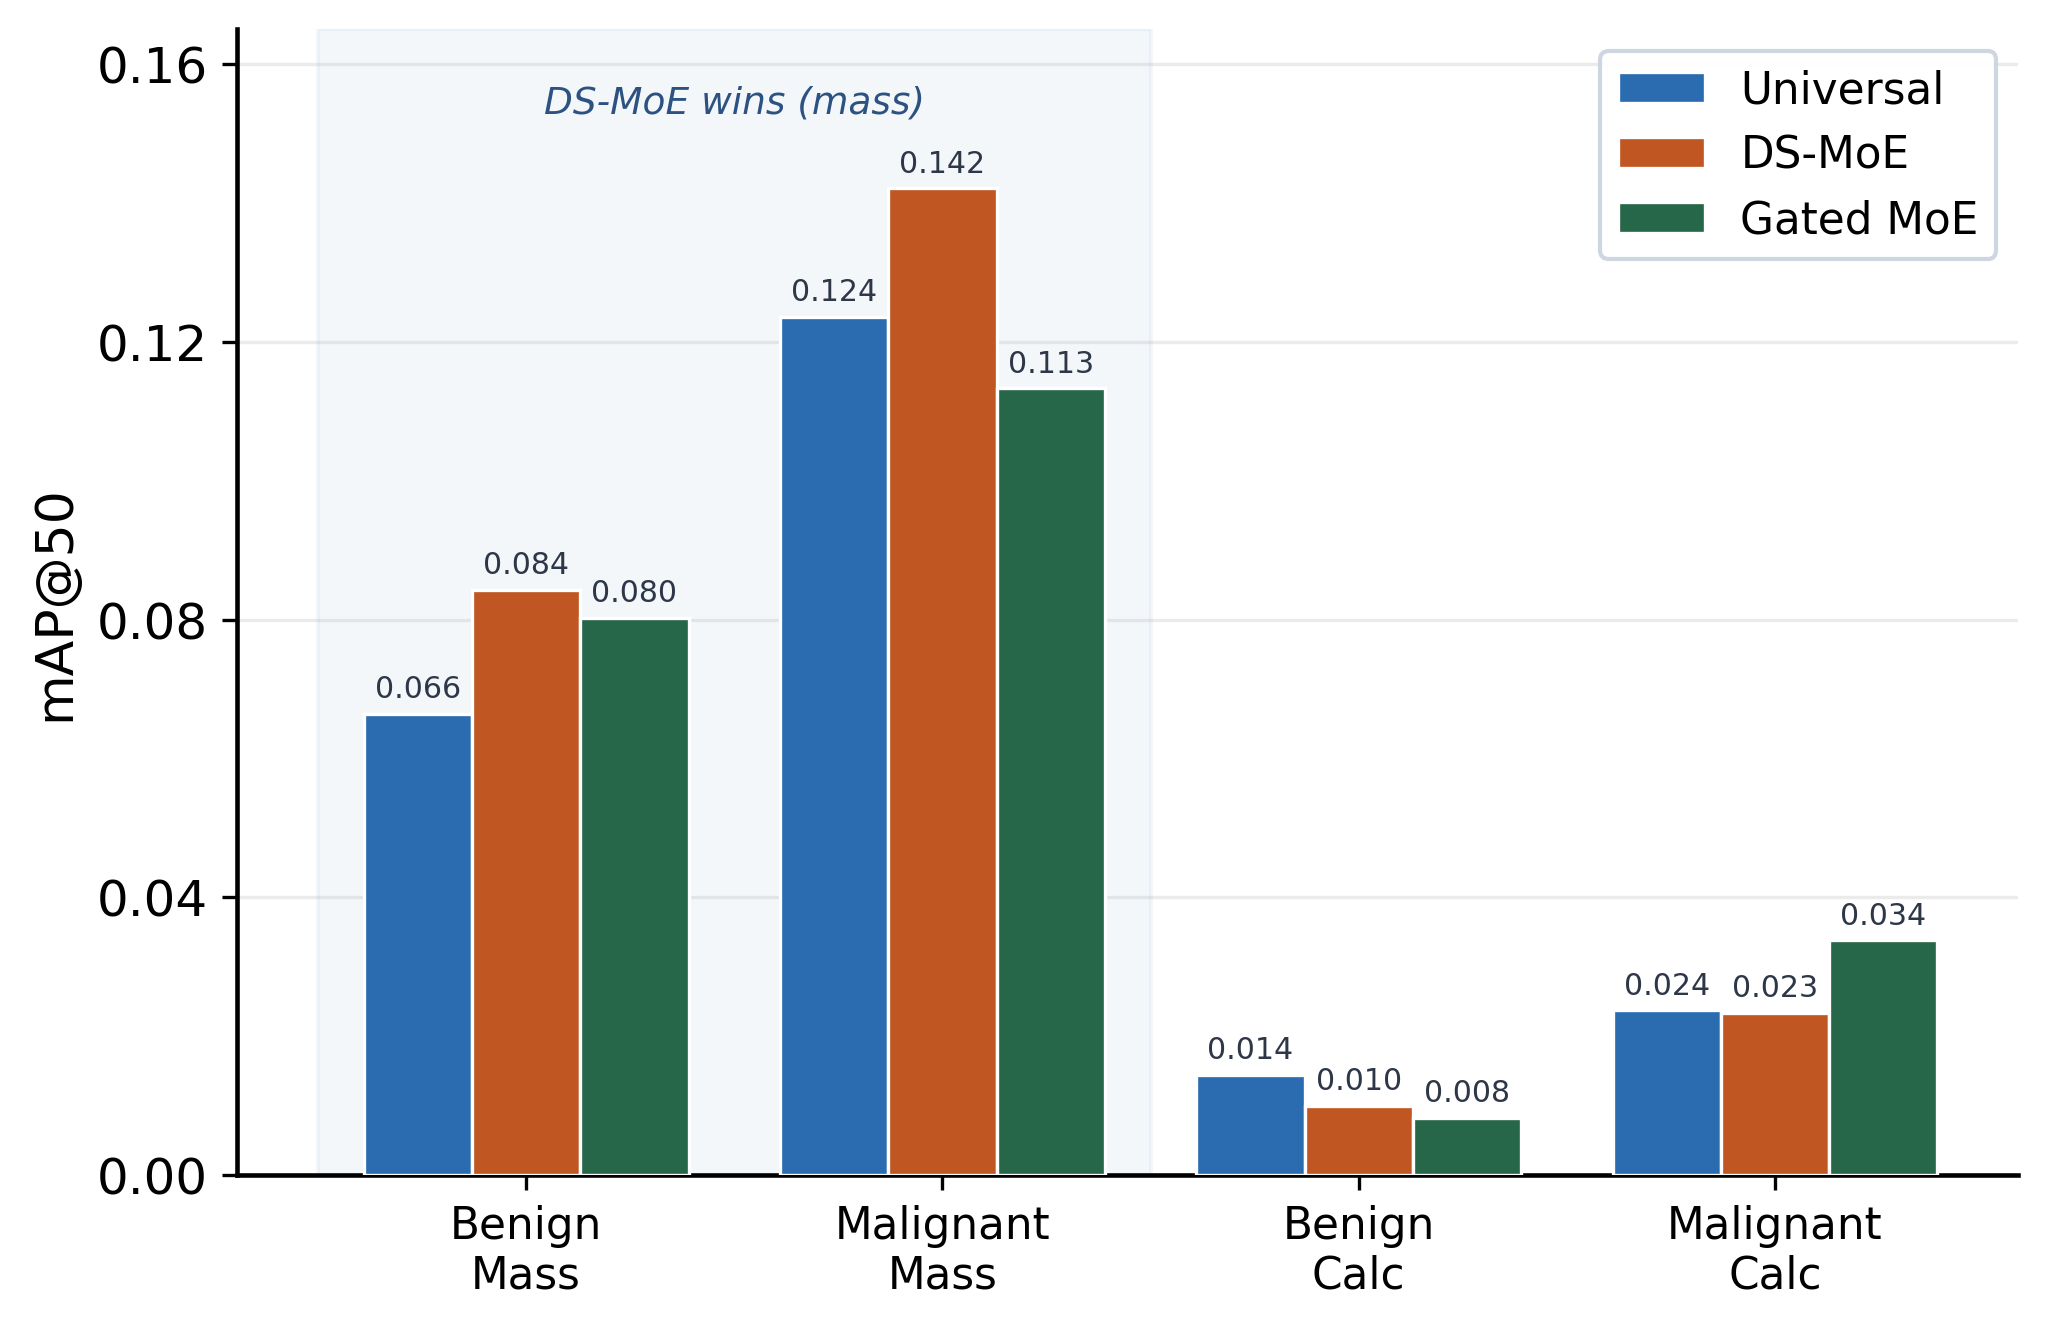
\includegraphics[width=0.84\columnwidth]{perclass_map.png}
\caption{Per-class mAP50 (mean over three seeds). Domain splitting
concentrates its gains on the two mass classes (shaded), where DS-MoE
clearly outperforms the universal baseline ($+27.0\%$ and $+15.0\%$),
while calcification performance remains uniformly low across all models,
identifying the calc expert as the system bottleneck.}
\label{fig:perclass}
\end{figure}

Tables~\ref{tab:perclass} and~\ref{tab:perclass_froc} decompose
performance into per-class contributions, visualised in
Fig.~\ref{fig:perclass}. DS-MoE wins on mAP50 for
mass classes (benign\_mass $+27.0\%$, malignant\_mass $+15.0\%$) while
Universal retains the advantage on per-class FROC S@2 across all four
classes (Section~\ref{sec:discussion} explains why this divergence
arises). Both calcification mAP50 classes are slightly worse under
DS-MoE, confirming that the calc expert introduces additional false
positives without proportional true positive gain---consistent with its
lower validation mAP50 of 0.167 versus 0.499 for the mass expert.

Gated MoE is higher on malignant\_calc mAP50 (0.0338 vs 0.0237), the
only class where it leads; given the small per-class values and $n=3$,
we treat this as suggestive rather than a reliable gating benefit.

\subsection{Per-Seed Results}

\begin{table}[tb]
\caption{Per-seed test results (458-image test set, IoU matching
threshold = 0.30 for FROC).}
\label{tab:perseed}
\centering
\begin{tabular}{llccc}
\toprule
\textbf{Seed} & \textbf{Model} & \textbf{mAP50} & \textbf{mAP50-95} & \textbf{FROC S@2}\\
\midrule
\multirow{3}{*}{42}
  & Universal  & 0.0556 & 0.0239 & 0.2027\\
  & DS-MoE     & 0.0519 & 0.0245 & 0.1873\\
  & Gated MoE  & 0.0484 & 0.0215 & 0.1737\\
\midrule
\multirow{3}{*}{1}
  & Universal  & 0.0590 & 0.0245 & 0.2104\\
  & DS-MoE     & 0.0798 & 0.0364 & 0.2066\\
  & Gated MoE  & 0.0660 & 0.0290 & 0.2046\\
\midrule
\multirow{3}{*}{123}
  & Universal  & 0.0564 & 0.0244 & 0.1931\\
  & DS-MoE     & 0.0631 & 0.0292 & 0.2143\\
  & Gated MoE  & 0.0621 & 0.0284 & 0.2066\\
\bottomrule
\end{tabular}
\end{table}

Table~\ref{tab:perseed} shows per-seed results. DS-MoE wins on mAP50
for seeds 1 and 123 but not seed 42 (whose mass expert had lower
validation mAP50), underscoring the seed-level variance behind the
within-noise aggregate gain.

\subsection{Ablation: CLAHE Preprocessing}
\label{sec:ablation}

\begin{table}[tb]
\caption{Effect of CLAHE preprocessing on the calcification expert
(seed 42, evaluated on the expert val partition; training converged at
121 epochs without CLAHE versus 55 with CLAHE). The No-CLAHE mAP50
(0.070) is this single seed; the three-seed mean is 0.167
(Table~\ref{tab:expert_val}), the gap reflecting the high variance of
the 17-image calc val partition.}
\label{tab:clahe}
\centering
\begin{tabular}{lccc}
\toprule
\textbf{Config} & \textbf{mAP50} & \textbf{Ben. Calc} & \textbf{Mal. Calc}\\
\midrule
No CLAHE (ours) & \textbf{0.070} & \textbf{0.060} & \textbf{0.080}\\
CLAHE ($c{=}2.0$, $8{\times}8$) & 0.043 & 0.023 & 0.063\\
$\Delta$ & $-$38.6\% & $-$61.7\% & $-$21.3\%\\
\bottomrule
\end{tabular}
\end{table}

Table~\ref{tab:clahe} reports the effect of Contrast Limited Adaptive
Histogram Equalisation (CLAHE) applied as preprocessing to the
calcification expert. CLAHE reduces mAP50 by 38.6\% (0.070 to 0.043)
and causes early stopping at epoch 55 versus 121 for the baseline,
indicating that CLAHE prevents model convergence. The explanation is
that CBIS-DDSM images are already preprocessed JPEGs; CLAHE distorts
the subtle pixel-level intensity patterns that YOLO uses to identify
calcification specks and disrupts the pretrained COCO feature maps.
This negative result, though observed for a single seed and a single
CLAHE setting ($c{=}2.0$, $8{\times}8$), is a useful practitioner
signal: CLAHE, while widely recommended in medical imaging preprocessing
pipelines, was harmful for YOLO-based calcification detection on the
already-JPEG-compressed CBIS-DDSM images in our setup, and warrants
caution rather than default application.

%-----------------------------------------------------------------------
\section{External Validation}
\label{sec:external}

\subsection{INbreast Zero-Shot Transfer}

\begin{table}[tb]
\caption{Zero-shot transfer to INbreast: mass-only FROC S@2
(116 GT boxes, 107 images). Calc excluded: INbreast uses point
annotations incompatible with cluster-level IoU $\geq 0.30$.}
\label{tab:inbreast}
\centering
\begin{tabular}{lccc}
\toprule
\textbf{Seed} & \textbf{Universal} & \textbf{DS-MoE} & \textbf{$\Delta$}\\
\midrule
42  & 0.7759 & 0.7759 & $+$0.0000\\
1   & 0.7328 & 0.8448 & $+$0.1121\\
123 & 0.7241 & 0.8707 & $+$0.1466\\
\midrule
Mean $\pm$ Std & $0.7443 \pm 0.0226$ & $\mathbf{0.8305 \pm 0.0400}$ & $+0.0862$\\
\bottomrule
\end{tabular}
\end{table}

INbreast \cite{moreira2012inbreast} is a full-field digital mammography
dataset acquired at a separate institution with different equipment.
We apply CBIS-DDSM-trained models directly without fine-tuning.
Calcification evaluation is excluded: INbreast annotates individual
calcification specks as point locations rather than cluster bounding
boxes, making cluster-level IoU $\geq 0.30$ structurally unmeasurable.
We report mass S@2 only on 116 ground-truth mass boxes from 107 images.

Table~\ref{tab:inbreast} shows DS-MoE achieves mean mass S@2 of
$0.8305 \pm 0.0400$ versus $0.7443 \pm 0.0226$ for Universal, a mean
improvement of $+0.0862$ (11.6\%). Seeds 1 and 123 show clear
advantages of $+0.11$ and $+0.15$. Seed 42 produces an exact tie at
0.7759, where both models detect exactly 90 of the 116 boxes at the 2
FP/image operating point---a FROC curve threshold coincidence, not
model equivalence. The mass specialisation advantage persists in
zero-shot transfer across acquisition modality (screen-film to digital),
confirming the benefit is not dataset-specific.

\subsection{MIAS}

The mini-MIAS dataset \cite{suckling1994mias} contains 322 images with
119 ground-truth boxes (53 benign mass, 39 malignant mass, 15 benign
calc, 12 malignant calc).
DS-MoE achieves mAP50 of $0.0917 \pm 0.0063$ versus $0.0880 \pm 0.0330$
for Universal ($+4.2\%$, consistent across all three seeds). Overall
FROC S@2 favours Universal ($0.4314 \pm 0.0241$ vs $0.3922 \pm 0.0317$);
however, only 27 calcification ground-truth boxes exist across 322
images, making FROC unreliable at this operating point. The consistent
mAP50 improvement confirms that mass specialisation generalises to
MIAS, a different screen-film dataset.

\subsection{CMMD}

The Chinese Mammography Database (CMMD) \cite{cui2021cmmd} provides
image-level cancer labels without bounding box annotations. We therefore measure
image-level detection sensitivity: a test image is counted as detected
if at least one prediction box is produced above the confidence
threshold. DS-MoE achieves image-level sensitivity of
$0.1548 \pm 0.0287$ versus $0.0020 \pm 0.0014$ for Universal. The
resulting 77-fold ratio is dominated by the near-zero denominator and
should be read alongside the absolute values: under this severe domain
shift (screen-film CBIS-DDSM to Chinese digital screening) the Universal
model detects almost nothing, whereas DS-MoE mass specialisation recovers
a modest but non-trivial fraction, indicating broader cross-scanner
generalisation. Note that image-level
sensitivity is a proxy metric in the absence of bounding box annotations;
localisation accuracy cannot be assessed on CMMD.

%-----------------------------------------------------------------------
\section{Discussion}
\label{sec:discussion}

The central finding is that domain specialisation substantially improves
mass detection precision (mAP50) while leaving calcification performance
largely unchanged, and that the calcification specialist is the limiting
component of the current system. At a 1280-pixel input, a microcalcification cluster of 5--15 pixels in
the original acquisition reduces to roughly 2--5 pixels---below the
reliable receptive field of standard anchors---and training on a
class-focused subset does not change this pixel budget.

\textbf{Per-class FROC regression.} Despite the aggregate FROC S@2 tie,
Table~\ref{tab:perclass_froc} shows that Universal outperforms DS-MoE on
all four per-class FROC metrics, with mass class losses of 14.7\% and
19.3\%. This apparent contradiction is explained by the inference design:
running both expert networks on every image doubles the total prediction
count before NMS. For mass-dominant images, the calc expert contributes
spurious false-positive boxes; these cross-domain FPs inflate the per-image
false-positive count for the mass class, shifting the per-class FROC
operating curve left and reducing the sensitivity achievable at the
2 FP/image threshold. The aggregate FROC tie arises because the FP
inflation from mass-dominant and calc-dominant images approximately
cancels across the mixed test set. This cross-expert contamination is
the primary limitation of the unconditional ``run all experts'' strategy
and motivates confidence gating as a direction---even though the current
71.2\% router accuracy is insufficient to recover the loss.

\textbf{Calcification bottleneck.} We investigated native-resolution
tiling (1024-pixel tiles with stride-4 P2 head) as an alternative.
This approach plateaued at validation mAP50 of approximately 0.07
because tiling discards global tissue context that is important for
calcification characterisation. Cluster boundaries are partially defined
by their relationship to surrounding parenchyma, and short tiles with
insufficient overlap lose this context. A useful calc expert likely
requires large-overlap tiling with SAHI \cite{akyon2022sahi} at inference,
or a dual-branch architecture combining high-resolution local crops with
a global context stream.

\textbf{External validity.} A zero-shot experiment on VinDr-Mammo
\cite{nguyen2023vindr} showed Universal outperforming DS-MoE; we report
this to avoid publication bias and attribute the finding to a domain gap
specific to Vietnamese digital screening mammography---a different
acquisition modality from CBIS-DDSM screen-film.

\textbf{Limitations.} Three seeds are a pilot; formal claims require
$\geq 10$ seeds, and the mAP50 gain ($+0.008$) is within one DS-MoE
standard deviation. The universal baseline is not capacity- or
FLOP-matched to DS-MoE (two detectors), so the mass-precision gain
cannot be fully separated from an ensemble/capacity effect; a
capacity-matched control is needed to isolate domain splitting. Router
accuracy (71.2\%) is insufficient for reliable gating, the calc expert
used full-image inference only, and CMMD is image-level only.

%-----------------------------------------------------------------------
\section{Conclusion}
\label{sec:conclusion}

We presented DS-MoE, a domain-split mixture-of-experts framework for
four-class mammography lesion detection. Specialist YOLO11l detectors
for mass and calcification subtypes are trained independently and merged
at inference through a class-offset union. On CBIS-DDSM, DS-MoE
achieves 13.9\% higher mAP50 than a leakage-free universal baseline
with mass class improvements of 27\% and 15\% (an effect within one
standard deviation that warrants more seeds to confirm). Aggregate FROC
S@2 is equivalent ($0.2027$ vs $0.2021$), but per-class FROC favours the
universal baseline; this per-class regression is identified as a
consequence of cross-domain false-positive inflation from the
unconditional dual-expert inference rather than a fundamental
sensitivity loss. Zero-shot validation on INbreast ($+11.6\%$ mass
FROC), MIAS ($+4.2\%$ mAP50), and CMMD (proxy image-level sensitivity
$0.002 \rightarrow 0.155$) suggests cross-scanner generalisation of the
mass specialist. The calcification expert is the identified bottleneck.

\noindent\textbf{Future work.} The calcification bottleneck motivates
resolution-aware inference---large-overlap SAHI tiling or a dual-branch
design coupling high-resolution local crops with a global context
stream---to recover the small-object sensitivity lost at 1280-pixel
input, alongside a stronger router for reliable gating and a larger seed
pool ($\geq 10$) for formal significance testing. To improve clinical
transparency, we plan to add interpretability through class-activation
heatmaps that visualise the image evidence underlying each expert's
predictions, and to extend the framework with a dedicated
benign-versus-malignant classification stage on the detected regions,
aiming to strengthen downstream diagnostic performance across further
multi-institution cohorts.

%-----------------------------------------------------------------------
\begin{thebibliography}{15}
\setlength{\itemsep}{0pt}
\setlength{\parskip}{0pt}

\bibitem{sung2021global}
H.~Sung \textit{et al.}, ``Global cancer statistics 2020,''
\textit{CA Cancer J. Clin.}, vol.~71, no.~3, pp.~209--249, 2021.

\bibitem{tabar2003swedish}
L.~Tabar \textit{et al.}, ``The Swedish two-county trial twenty years
later,'' \textit{Radiol. Clin. North Am.}, vol.~38, no.~4,
pp.~625--651, 2000.

\bibitem{doi2007computer}
K.~Doi, ``Computer-aided diagnosis in medical imaging,''
\textit{Comput. Med. Imaging Graph.}, vol.~31, pp.~198--211, 2007.

\bibitem{lee2017curated}
R.~S.~Lee \textit{et al.}, ``A curated mammography data set for use in
computer-aided detection and diagnosis research,''
\textit{Sci. Data}, vol.~4, Art.~no.~170177, 2017.

\bibitem{moreira2012inbreast}
I.~C.~Moreira \textit{et al.}, ``INbreast: Toward a full-field digital
mammographic database,'' \textit{Acad. Radiol.}, vol.~19, no.~2,
pp.~236--248, 2012.

\bibitem{ribli2018detecting}
D.~Ribli \textit{et al.}, ``Detecting and classifying lesions in
mammograms with deep learning,'' \textit{Sci. Rep.}, vol.~8,
Art.~no.~4165, 2018.

\bibitem{redmon2016you}
J.~Redmon \textit{et al.}, ``You only look once: Unified, real-time
object detection,'' in \textit{Proc. IEEE CVPR}, 2016, pp.~779--788.

\bibitem{jocher2024ultralytics}
G.~Jocher, J.~Qiu, and A.~Chaurasia, ``Ultralytics YOLO,'' 2024.
[Online]. Available: https://github.com/ultralytics/ultralytics

\bibitem{akyon2022sahi}
F.~C.~Akyon, S.~O.~Altinuc, and A.~Temizel, ``Slicing aided hyper
inference and fine-tuning for small object detection,'' in
\textit{Proc. IEEE ICIP}, 2022, pp.~966--970.

\bibitem{jacobs1991adaptive}
R.~A.~Jacobs \textit{et al.}, ``Adaptive mixtures of local experts,''
\textit{Neural Comput.}, vol.~3, no.~1, pp.~79--87, 1991.

\bibitem{shazeer2017outrageously}
N.~Shazeer \textit{et al.}, ``Outrageously large neural networks,''
in \textit{Proc. ICLR}, 2017.

\bibitem{pedregosa2011scikit}
F.~Pedregosa \textit{et al.}, ``Scikit-learn: Machine learning in
Python,'' \textit{J. Mach. Learn. Res.}, vol.~12,
pp.~2825--2830, 2011.

\bibitem{nguyen2023vindr}
H.~T.~Nguyen \textit{et al.}, ``VinDr-Mammo: A large-scale benchmark
dataset,'' \textit{Sci. Data}, vol.~10, Art.~no.~277, 2023.

\bibitem{suckling1994mias}
J.~Suckling \textit{et al.}, ``The Mammographic Image Analysis Society
digital mammogram database,'' in \textit{Proc. 2nd Int. Workshop Digital
Mammography}, 1994, pp.~375--378.

\bibitem{cui2021cmmd}
C.~Cui \textit{et al.}, ``The Chinese Mammography Database (CMMD),''
The Cancer Imaging Archive, 2021.

\end{thebibliography}

\end{document}
